\chapter{Paralelné komunikujúce systémy gramatík ($PCGS$)}

Dostávame sa k ďalšiemu typu paralelizmu. Paralelný komunikujúci
systém gramatík v sebe integruje viacero gramatík nejakého typu,
ktoré sú zosynchronizované podľa akýchsi globálnych hodín, takže
pracujú v taktoch. Označme si tieto gramatiky $G_1,G_2,\dots
,G_n$. Každá z týchto gramatík pracuje na svojej vetnej forme
podľa svojich pravidiel. Naviac týmto gramatikám dodáme špeciálny
neterminál $Q$ ($query$ symbol). Ak sa vo vetnej forme nejakej
gramatiky vyskytne symbol $Q_i$, znamená to, že v ďalšom takte sa
$Q_i$ zmení na vetnú formu vygenerovanú gramatikou $G_i$, pričom
$G_i$ začne generovať odznova. Toto presunutie sa vykoná len
vtedy, keď vetná forma $G_i$ neobsahuje, žiadny symbol $query$.
Teraz pristúpime k formálnemu zadefinovaniu tohto modelu.

\section{Definície a označenia}

\begin{definicia}
  $PCGS$ (Parallel Communicating Grammar Systems) stupňa $n$
  je\newline $(n+3)$-ica $\Gamma =(N,K,T,G_1,\dots ,G_n)$ kde $N$ je
  množina neterminálov, $K$ je množina\linebreak komunikačných
  \mbox{$(query)$} symbolov štandardne označovaných $K=\{Q_1,\dots
  ,Q_n\}$, $T$ je množina terminálov, pre každé $i$ $G_i=(N\cup
  K,T,P_i,S_i)$ sú bez-$\varepsilon$ gramatiky ľubovoľného
  typu\footnote{väčšinou sa používajú regulárne alebo bezkontextové
  typy gramatík, lebo pri zložitejších typoch už máme veľké problémy
  sledovať, čo taký systém vôbec robí}, pričom $S_i\in N$ je
  počiatočný neterminál a v $P_i$ nie sú pravidlá obsahujúce na
  ľavej strane $query$.
\end{definicia}

\begin{oznacenie}
  $V_\Gamma=N\cup K\cup T$
\end{oznacenie}

\begin{definicia}
  $n$-vetná forma (konfigurácia) je n-tica slov $(x_1,\dots ,x_n)$
  kde $x_i\in V_\Gamma^*$.
\end{definicia}

\begin{definicia}
  Krok odvodenia je relácia $\underset{\Gamma}\Ra$ na $n$-vetných
  formách definovaná nasledovne: $(x_1,\dots
  ,x_n)\underset{\Gamma}\Ra (y_1,\dots ,y_n)$ práve vtedy keď
  nastane jeden z prípadov:
  \begin{enumerate}
    \item (prepisovací krok) $x_i$ neobsahuje $query$ symbol a
      \begin{itemize}
        \item $x_i$ obsahuje neterminál, potom $x_i\underset{G_i}\Ra y_i$
        \item $x_i$ je terminálne slovo, potom $y_i=x_i$
      \end{itemize}
    \item (komunikačný krok) $x_i$ obsahuje $query$ symboly $Q_{j_1},\dots ,Q_{j_s}$ potom
      \begin{itemize}
        \item ak $x_{j_k}$ neobsahuje $query$ symbol, tak v $x_i$ nahradíme
        $Q_{j_k}$ vetnou formou $x_{j_k}$ a \mbox{$y_{j_k}=S_{j_k}$}
        \item ak $x_{j_k}$ obsahuje nejaký $query$ symbol tak v $x_i$ necháme $Q_{j_k}$
      \end{itemize}
      pre všetky ostatné $x_i$ neobsahujúce $query$ symboly platí
      $y_i=x_i$.
  \end{enumerate}
\end{definicia}

Práve vyslovená definícia je trochu komplikovaná, pretože neberie
do úvahy nejaký konkrétny typ gramatiky, ale je použiteľná pre
akýkoľvek typ gramatiky Chomskeho hierarchie. Keďže v ďalšom sa
budeme zaoberať hlavne $PCGS$ s regulárnymi komponentami,
vyslovíme teraz definíciu kroku odvodenia pre tieto $PCGS$, ktorá
je o niečo jednoduchšia.

\begin{definicia}
  Krok odvodenia je relácia $\underset{\Gamma}\Ra$ na $n$-vetných
  formách definovaná nasledovne: $(x_1,\dots
  ,x_n)\underset{\Gamma}\Ra (y_1,\dots ,y_n)$ práve vtedy keď
  nastane jeden z prípadov:
  \begin{enumerate}
    \item $x_i$ neobsahuje $query$ symbol, teda
    \begin{itemize}
      \item $x_i=w_iA$ kde $w_i\in T^*$ a $A\in N$, potom $x_i\underset{G_i}\Ra y_i$
      \item $x_i=w_i$ je terminálne slovo, potom $y_i=x_i$
    \end{itemize}
    \item $x_i$ obsahuje $query$ symbol, teda $x_i=w_iQ_j$, a potom
    \begin{itemize}
      \item ak $x_j$ neobsahuje $query$ symbol, tak $y_i=w_ix_j$ a $y_j=S_j$
      \item ak $x_j$ obsahuje nejaký $query$ symbol, tak $y_i=x_i$
    \end{itemize}
    pre všetky ostatné $x_i$ neobsahujúce $query$ symboly platí
    $y_i=x_i$
  \end{enumerate}
\end{definicia}

Uvedomme si, že odvodenie v $PCGS$ pozostáva z prepisovacích a
komunikačných krokov. Prepisovací krok nastane vtedy, ak
sa v n-vetnej forme nevyskytuje ani jeden komunikačný symbol, a
potom všetky gramatiky spravia jeden krok odvodenia na svojich
vetných formách. Ak nejaký komponent n-vetnej formy je terminálne
slovo, tak sa v ďalšom nemení až kým nejaká gramatika nepožiada o
jej obsah. Ak sa v nejakej vetnej forme vyskytne neterminál, ktorý
sa nedá prepisať, tak sa odvodenie zasekne. V komunikačnom kroku
sa nahradia všetky $query$ príslušnými vetnými formami, ak tie
neobsahujú $query$. Je zrejmé, že komunikačných krokov môže po
sebe nasledovať viac, až kým sa celá n-vetná forma ``nevyčistí''
od $query$. Môže sa stať, že komunikácia sa zacyklí a nebude možné
vykonať žiaden prepisovací krok. Vtedy sa odvodenie zasekne.

\begin{definicia}
  Jazyk generovaný $PCGS$ systémom $\Gamma$ je množina terminálnych
  slov vygenerovaných gramatikou $G_1$. Teda
  $L(\Gamma)=\{x\in T^*\mm (S_1,\dots
  ,S_n)\overset{*}{\underset{\Gamma}\Ra} (x,v_2,\dots ,v_n),v_i\in
  V_\Gamma^*\}$.
\end{definicia}

\section{Parametre uvažované na $PCGS$}

\begin{enumerate}
  \item komunikačná štruktúra - Môžeme si predstaviť orientovaný graf, ktorého
    vrcholy sú gramatiky a hrana z $G_i$ vedie do $G_j$ ak $G_i$ môže
    generovať $Q_j$. Komunikačné štruktúry delíme na dva základné
    typy:
    \begin{description}
      \item{centralizované} - $query$ môže generovať len gramatika $G_1$
      \item{necentralizované} - všetky ostatné napr. dag(directed acyclic
      graph), tree, two-way array, one-way array, two-way ring, one-way
      ring, $\dots$
    \end{description}
  \item typ gramatík v komponentoch
  \item počet komponentov (gramatík)
  \item počet komunikačných krokov
  \item systémy s resetom resp. bez resetu - t.j. či sa vetná forma
    po presunutí svojho obsahu do inej vetnej formy zmení na
    počiatočný neterminál alebo nie.
\end{enumerate}

\begin{figure}[t]
  \centering
  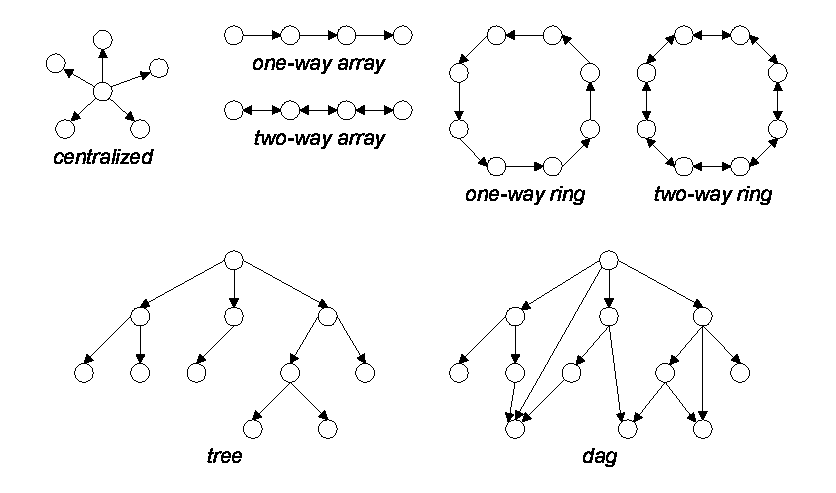
\includegraphics{img/pcgs/structur}
  \caption{Príklady komunikačných štruktúr $PCGS$} \label{pcgs_obr_structures}
\end{figure}

\begin{oznacenie}
  $xPCGS_nX$ - trieda $PCGS$-systémov kde
  $x\in\{centr,tree,dag,\dots\}$ je typ komunikačnej
  štruktúry\footnote{ak nie je uvedený typ komunikačnej štruktúry,
  máme na mysli triedu všetkých $PCGS$-systémov bez ohľadu na
  štruktúru}, $n$ je počet komponentov ($(n=*)$ označuje ľubolný
  počet komponentov) a $X\in\{REG,LIN,CF,\dots\}$ je typ
  komponentov\footnote{lineárne gramatiky (LIN) sú bezkontextové
  gramatiky, ktoré majú na pravej strane pravidiel najviac jeden
  neterminál}.
\end{oznacenie}

\section{Generatívna sila $PCGS$}

Na bližšie pochopenie sily $PCGS$ si uvedieme najskôr zopár
príkladov.

\begin{priklad}
  \label{pcgs_prikl_1}
  $\Gamma_1=(\{S_1,S_2,S_3\},K,\{a,b,c\},G_1,G_2,G_3)$, kde množiny
  pravidiel príslušných gramatík sú:
  \begin{itemize}
    \item $P_1=\{S_1\ra aS_1,S_1\ra aQ_2,S_2\ra
    bQ_3,S_3\ra c\}$
    \item $P_2=\{S_2\ra bS_2\}$
    \item $P_3=\{S_3\ra cS_3\}$
  \end{itemize}
  Skúsme si napísať pár krokov odvodenia: \\ $(S_1,S_2,S_3)\Ra
  (aS_1,bS_2,cS_3)\Ra\dots k-krokov\dots\Ra
  (a^kS_1,b^kS_2,c^kS_3)\Ra\newline
  (a^{k+1}Q_2,b^{k+1}S_2,c^{k+1}S_3)\Ra
  (a^{k+1}b^{k+1}S_2,S_2,c^{k+1}S_3)\Ra
  (a^{k+1}b^{k+2}Q_3,bS_2,c^{k+2}S_3)\Ra\newline
  (a^{k+1}b^{k+2}c^{k+2}S_3,bS_2,S_3)\Ra
  (a^{k+1}b^{k+2}c^{k+3},b^2S_2,cS_3)$ \\ Teraz už vidíme, že
  $L(\Gamma_1)=\{a^nb^{n+1}c^{n+2}\mm n\geq 1\}$, a teda
  centralizovaný $PCGS$ s troma re\-gu\-lárnymi komponentami
  vygeneroval jazyk, ktorý nie je regulárny, ba dokonca ani
  bezkontextový.
\end{priklad}

\begin{priklad}
  \label{pcgs_prikl_2} $\Gamma_2=(\{S_1,S_2,A\},K,\{a,b,c\},G_1,G_2)$,
  kde
  \begin{itemize}
    \item $P_1=\{S_1\ra aS_1,S_1\ra Q_2,A\ra
    aS_1,A\ra c\}$
    \item $P_2=\{S_2\ra A,A\ra bA\}$
  \end{itemize}
  Napíšme si pár krokov odvodenia: \\ $(S_1,S_2)\Ra
  (aS_1,A)\overset{*}\Ra (a^kS_1,b^{k-1}A)\Ra (a^k Q_2, b^k A)\Ra
  (a^k b^k A, S_2)\Ra (a^k b^k aS_1,A)\Ra \dots$
  \\ Ľahko vidno, že $L(\Gamma_2)=(\{a^nb^n\mm
  n\geq 1\})^+c$, čo je opäť jazyk, ktorý nie je ani bezkontextový.
\end{priklad}

\begin{priklad}
  \label{pcgs_prikl_3} $\Gamma_3=(\{S_1,S_2\},K,\{a,b,c,d\},G_1,G_2)$
  \begin{itemize}
    \item $P_1=\{S_1\ra cS_1d,S_1\ra cQ_2d\}$
    \item $P_2=\{S_2\ra aS_2b,S_2\ra ab\}$
  \end{itemize}
  Všimnime si niektoré možné odvodenia:
  \begin{enumerate}
    \item $(S_1,S_2)\overset{*}\Ra
    (c^{k-1}S_1d^{k-1},a^{k-1}S_2b^{k-1})\Ra (c^kQ_2d^k,a^kS_2b^k)\Ra
    (c^ka^kS_2b^kd^k,S_2)$ a tu sa $\Gamma_3$ zasekne
    \item $(S_1,S_2)\overset{*}\Ra
    (c^{k-1}S_1d^{k-1},a^{k-1}S_2b^{k-1})\Ra (c^kQ_2d^k,a^kb^k)\Ra
    (c^ka^kb^kd^k,S_2)$
    \item $(S_1,S_2)\overset{*}\Ra
    (c^{k-1}S_1d^{k-1},a^{k-1}S_2b^{k-1})\Ra
    (c^kS_1d^k,a^kb^k)\overset{*}\Ra
    (c^{k+i}Q_2d^{k+i},a^kb^k)\Ra\newline
    (c^{k+i}a^kb^kd^{k+i},a^kb^k)$
  \end{enumerate}
  Teda $L(\Gamma_3)=\{c^la^kb^kd^l\mm l\geq k\geq 1\}$. $PCGS$ s
  dvoma lineárnymi komponentami vygeneroval jazyk mimo bezkontextovú
  triedu jazykov.
\end{priklad}

\begin{priklad}
  $\Gamma_4=(\{S_1,S_2\},K,\{a,b,c\},G_1,G_2)$
  \begin{itemize}
    \item $P_1=\{S_1\ra S_1,S_1\ra Q_2cQ_2\}$
    \item $P_2=\{S_2\ra aS_2,S_2\ra bS_2,S_2\ra
    a,S_2\ra b\}$
  \end{itemize}
  Ľahko vidno, že $L(\Gamma_4)=\{wcw\mm w\in\{a,b\}^+\}$, a teda
  $PCGS$ s dvoma bezkontextovými komponentami vygeneroval jazyk,
  ktorý nie je bezkontextový.
\end{priklad}

\begin{priklad}
  $\Gamma_5=(\{S_1,S_2,S_3\},K,\{a,b,c,d\},G_1,G_2,G_3)$
  \begin{itemize}
    \item $P_1=\{S_1\ra aS_1,S_2\ra aQ_2,S_3\ra d\}$
    \item $P_2=\{S_2\ra bS_2,S_2\ra bQ_3\}$
    \item $P_3=\{S_3\ra cS_3\}$
  \end{itemize}
  Všimnime si odvodenie, v ktorom nasleduje po sebe viac
  komunikačných krokov:
  \\ $(S_1,S_2,S_3)\overset{*}\Ra (a^kS_1,b^kS_2,c^kS_3)\Ra
  (a^{k+1}Q_2,b^{k+1}Q_3,c^{k+1}S_3)\Ra
  (a^{k+1}Q_2,b^{k+1}c^{k+1}S_3,S_3)\Ra
  (a^{k+1}b^{k+1}c^{k+1}S_3,S_2,S_3)\Ra
  (a^{k+1}b^{k+1}c^{k+1}d,bS_2,cS_3)$ \\ Ľahko vidno, že
  $L(\Gamma_5)=\{a^nb^nc^nd\mm n\geq 1\}\in
  \Langclass{CS}-\Langclass{CF}$.
\end{priklad}

\begin{priklad}
  V tomto príklade ukážeme ako $PCGS$ naplno využije silu svojej
  komunikácie a vyrobíme jazyk $L(\Gamma)=\{ w^{2^n}c\mm w\in\{
  a,b\}^*,n\geq 1\}$:
  \\ $\Gamma_6=(\{ S_1,S_2,S_3\} ,K,\{ a,b\} ,G_1,G_2,G_3)$
  \begin{itemize}
    \item $P_1=\{S_1\ra aS_1,S_1\ra bS_1,S_1\ra
    Q_2, \omega_1\ra Q_3,\omega_2\ra S_1',S_1'\ra c\}$
    \item $P_2=\{S_2\ra S_2,S_2\ra Q_1,S_1\ra\omega_1,
    S_1'\ra\omega_1\}$
    \item $P_3=\{S_3\ra S_3,S_3\ra Q_1,S_1\ra\omega_1,
    \omega_1\ra\omega_2,S_1'\ra\omega_1\}$
  \end{itemize}
  Pozrime sa na to ako funguje odvodenie v $\Gamma$:
  \\ $(S_1,S_2,S_3)\overset{*}\Ra (wS_1,S_2,S_3)
  \Ra (wS_1,Q_1,Q_1)\Ra (S_1,wS_1,wS_1)\Ra
  (Q_2,w\omega_1,w\omega_1)\Ra\newline (w\omega_1,S_2,w\omega_1)\Ra
  (wQ_3,S_2,w\omega_2)\Ra (ww\omega_2,S_2,S_3)\Ra
  (wwS_1',Q_1,Q_1)\overset{*}\Ra (w^4S_1',Q_1,Q_1)\overset{*}\Ra
  (w^{2^n}S_1',S_2,S_3)\Ra (w^{2^n}c,\dots )$
  \\ Pravidlá v $\Gamma$ sú zostavené tak dômyselne, že gramatiky
  $G_2$, $G_3$ naraz vygenerujú komunikačný symbol $Q_1$, teda
  prenesú si vetnú formu vygenerovanú prvou gramatikou a následne
  $G_1$ požiada o vetné formy $G_2$ a $G_3$, teda obsah vetnej formy
  $G_1$ sa zdvojnásobí. Ak by gramatiky takto ``nespolupracovali'',
  tak sa $\Gamma$ zasekne.
  \\ Všimnime si ešte, že $\Gamma$ vygeneruje slovo $w^{2^n}c$ v
  čase $O(n)$. $G_1$ na začiatku vygeneruje $w$ a potom pri každom
  zdvojnásobení $\Gamma$ používa už len konštantný počet krokov
  odvodenia. Treba si uvedomiť, že je to možné len vďaka tomu, že
  pri modeli $PCGS$ máme komunikáciu v podstate zadarmo, lebo v
  jednom kroku dokážeme preniesť ľubovoľne veľké slovo.
\end{priklad}

\begin{veta}
  Niekoľko porovnaní $PCGS$ s triedami Chomského hierarchie:
  \begin{enumerate}
    \item $\Langclass{PCGS_n REG}-\Langclass{LIN}\neq\emptyset$ pre $n\geq 2$
    \item $\Langclass{PCGS_n REG}-\Langclass{CF}\neq\emptyset$ pre $n\geq 3$
    \item $\Langclass{PCGS_n LIN}-\Langclass{CF}\neq\emptyset$ pre $n\geq 2$
  \end{enumerate}
\end{veta}

\begin{dokaz}
  Pozri príklady \ref{pcgs_prikl_2}, \ref{pcgs_prikl_1} a \ref{pcgs_prikl_3}.
\end{dokaz}

\begin{veta}
  \label{pcgs_veta_LLINtoLcentrPCGS*REG}
  $\Langclass{LIN}-\Langclass{centrPCGS_* REG}\neq\emptyset$
\end{veta}

\begin{dokaz}
  Uvažujme jazyk $L=\{a^nb^mcb^ma^n\mm n,m\geq 1\}$. \\ Zrejme
  $L \in \Langclass{LIN}$. Ukážeme, že
  $L \not\in \Langclass{centrPCGS_* REG}$. \\ Bez ujmy na všeobecnosti
  môžme predpokladať, že $G_1$ negeneruje $a$-čka, lebo ak by
  generovala tak to isté dokáže aj iný komponent a $G_1$ môže
  požiadať o jej výstup. Teda $a$-čka generujú dve iné gramatiky
  ($G_2,G_3$), lebo potrebujeme rovnaký počet $a$-čiek na začiatku
  aj na konci vetnej formy. Podobne musia existovať aj dve gramatiky
  ($G_4,G_5$) na generovanie $b$-čiek. Ak po nejakom počte krokov
  $G_1$ vygeneruje $Q_2$, tak v konečnom (dosť malom) počte krokov
  musí vygenerovať aj $Q_3$, lebo $G_3$ sa nemá ako dozvedieť, že už
  nemá generovať $a$-čka, keďže uvažujeme centralizovanú komunikačnú
  štruktúru. Z toho ale plynie, že v tomto konečnom počte krokov
  musí $G_1$ vygenerovať $Q_4$ a $Q_5$, lebo uvažujeme regulárne
  gramatiky. Teda $G_4$ a $G_5$ majú obmedzený čas na generovanie
  $b$-čiek, a teda počet $b$-čiek nemôže byť oveľa
  väčší\footnote{$m$ môže byť väčšie od $n$ najviac lineárne v
  závislosti od pravidiel v $G_2,G_3$ a v $G_4,G_5$} ako počet
  $a$-čiek, čo je spor s tým, že potrebujeme vygenerovať aj slová s
  ľubovoľne veľkým rozdielom medzi $m$ a $n$.
\end{dokaz}

\pagebreak

\begin{veta}
  $\Langclass{centrPCGS_2 REG} \subsetneq \Langclass{CF}$
\end{veta}

\begin{dokaz}
  Podľa vety \ref{pcgs_veta_LLINtoLcentrPCGS*REG} stačí dokázať už len
  inklúziu $\subseteq$:
  \\ Majme $\Gamma=(N,K,T,G_1,G_2)\in centrPCGS_2REG$. Chceme
  zostrojiť bezkontextovú gramatiku $G=(N',T,P,S)$ takú, že
  $L(\Gamma)=L(G)$. Rozšírime množinu neterminálov takto:\\
  $N'=N\cup \{[A,B]\mm A\in N,B\in N\}\cup\{\overline{A}\mm A\in
  N\}$, neskôr si ukážeme ako tieto nové neterminály budeme
  využívať. Najskôr sa zamyslime nad tým, ako bude vyzerať výsledné
  slovo $w\in L(\Gamma)$.\linebreak $w$ bude mať nasledujúce
  vlastnosti (obr.\ref{pcgs_obr_l2reglcf}):

  \begin{enumerate}
    \item $w$ sa dá dekomponovať na $w=w_1w_2\dots w_s$ pre nejaké $s\geq 1$
    \item $\forall i\; w_i=v_{i_1}v_{i_2}$ pričom $v_{i_1}$ generuje $G_1$
    a $v_{i_2}$ generuje $G_2$
    \item $v_{i_1}$ a $v_{i_2}$ sú generované na rovnaký počet
    krokov
  \end{enumerate}

  \begin{figure}[ht]
    \centering
    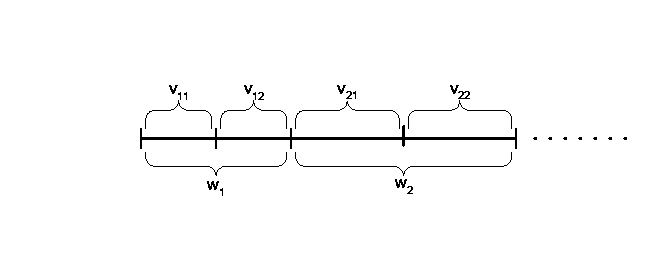
\includegraphics{img/pcgs/l2reglcf}
    \caption{Tvar slova generovaného $centrPCGS_2REG$}\label{pcgs_obr_l2reglcf}
  \end{figure}

  $G$ musí byť schopná generovať slová s takýmito vlastnosťami. Na
  zabezpečenie podmienky 3 bude $G$ generovať jednotlivé podslová
  $w_i$ odstredu t.j. nejaký špeciálny neterminál sa bude postupne
  obklopovať terminálmi podľa pravidiel $G_1,G_2$.
  \\ V $P$ budú pravidlá:
  \begin{description}
    \item{$S\ra [S_1,B] B$  $\forall B\in N$} \\Teda máme špeciálnu
    sadu neterminálov $[S_1,B]$, ktoré určujú, že podslovo $v_{1_1}$
    sa začína generovať z počiatočného neterminálu $S_1$ a podslovo
    $v_{1_2}$ bude mať posledný neterminál $B$. To v podstate znamená,
    že $G$ sa nedeterministicky rozhodne pre neterminál $B$.
    \item{$[A,B]\ra a[A',B']b$  ak $A\ra aA'\in P_1$ a $B'\ra bB\in
    P_2$} \\ Tieto pravidlá nám zabezpečujú postupné simulovanie
    odvodenia slov $v_{i_1}$ odpredu a slov $v_{i_2}$ odzadu, pričom
    toto odvodenie bude legálne vzhľadom na pravidlá $G_1,G_2$.
    \item{$[Q_2,S_2]\ra\varepsilon$} \\ Toto pravidlo zabezpečuje, že
    ak $G$ na začiatku dobre uhádla posledný neterminál $v_{i_2}$, tak
    po konečnom počte krokov simulácia $G_1$ dospela ku komunikačnému
    neterminálu $Q_2$ a simulácia $G_2$ v spätnom odvodení dospela k
    počiatočnému neterminálu $S_2$, teda neterminál $[Q_2,S_2]$ sa už
    nebude ďalej rozvíjať, a teda ho vymažeme.
    \item{$A\ra [A,B]B$  $\forall A,B\in N$} \\ Tieto pravidlá slúžia na
    správne nadväzovanie podslov $w_i$, $w_{i+1}$. To znamená, že
    týmto pravidlom $G$ uhádne akým neterminálom bude končiť ďalšie
    podslovo.
  \end{description}
  Ukážme si teraz ako funguje simulácia. Zoberme si nejaké odvodenie
  v $\Gamma$.
  \\ $(S_1,S_2)\Ra (u_1A_1,v_1B_1)\overset{*}\Ra (u_1u_2\dots u_kQ_2,v_1v_2\dots
  v_kB_k)\Ra (u_1\dots u_kv_1\dots v_kB_k,S_2)\Ra\dots$
  \\ Príslušná časť odvodenia v $G$ bude vyzerať takto:
  \\ $S\Ra [S_1,B_k]B_k\Ra u_1[A_1,B_{k-1}]v_kB_k\Ra u_1u_2[A_2,B_{k-2}]v_{k-1}v_kB_k
  \overset{*}\Ra\newline u_1\dots u_k[Q_2,S_2]v_1\dots v_kB_k\Ra
  u_1\dots u_kv_1\dots v_kB_k\Ra\dots$
  \\ $G$ najskôr nedeterministicky vybrala pravidlo $S\ra
  [S_1,B_k]B_k$ tak, aby správne uhádla neterminál, ktorým bude
  ďalej pokračovať $G_1$ v odvodení po komunikačnom kroku (t.j.
  neterminál, ktorý bol prenášaný v komunikačnom kroku). Potom
  postupne simulovala odvodenie $G_1$, $G_2$ a nakoniec vymazala
  neterminál $[Q_2,S_2]$ z vetnej formy. Takto ostal vo vetnej forme
  len neterminál $B_k$, ktorým začne ďalšiu simuláciu $G_1$. Teraz
  $G$ použije nejaké z pravidiel $B_k\ra [B_k,B]B$ na uhádnutie
  neterminálu, ktorý bude prenášaný v nasledujúcom komunikačnom
  kroku atď.

  \smallskip

  Ešte sa musíme zamyslieť nad tým, ako simuláciu ukončiť. Môžu
  nastať dva prípady:
  \begin{enumerate}
    \item $G_1$ už nepožiada $G_2$ o jej vetnú formu (teda nevyprodukuje $Q_2$)
    a sama vyprodukuje terminálne slovo. Pre túto možnosť dodáme do
    $P$ tieto pravidlá:
    \begin{itemize}
      \item $B\ra \overline{B}$  $\forall B\in N$
      \item $\overline{A}\ra u\overline{B}$ ak $A\ra uB\in P_1$
    \end{itemize}
    Tým, že sme použili ``pruhované'' neterminály a nemáme pravidlo
    typu $\overline{A}\ra A$ sme zmarili ďalšiu\footnote{k dispozícii
    máme samozrejme aj pravidlo $S\ra\overline{S}$ teda
    žiadna komunikácia nemusí nastať} komunikáciu, a teda simulujeme
    $G_1$ až kým nevygeneruje terminálne slovo.
    \item $G_2$ skončí skôr (t.j. vygeneruje terminálne slovo) ako
    $G_1$ požiada o jej vetnú formu. V $\Gamma$ sa vetná forma $G_2$
    nemení a čaká, kým $G_1$ vygeneruje $Q_2$. Pre túto možnosť dodáme
    do $P$ tieto pravidlá:
    \begin{itemize}
      \item $A\ra [A,\varepsilon]$  $\forall A\in N$
      \item $[A,\varepsilon]\ra u[A',\varepsilon]$ ak $A\ra uA'\in P_1$
      \item $[A,\varepsilon]\ra u[A',B]$  $\forall B\in N$ ak $A\ra uA'\in P_1$
    \end{itemize}
  Teda pravidlá typu $[A,\varepsilon]\ra u[A',\varepsilon]$ simulujú
  čakaknie $G_2$ na komunikáciu a pravidlá typu $[A,\varepsilon]\ra
  u[A',B]$ opäť slúžia na uhádnutie posledného neterminálu, ktorý sa
  objavil vo vetnej forme $G_2$.
  \end{enumerate}
\end{dokaz}

\begin{lema}[Pumpovacia lema pre $centrPCGS_nREG$]
  \label{pcgs_lema_pumplemacentrPCGSnREG}

  Nech $L \in \Langclass{centrPCGS_n REG}$.
  Potom existuje prirodzené číslo $M$, že
  $\forall w\in L$ také, že\linebreak $|w|>M$ existuje $m$ $1\leq
  m\leq n$ a existujú $x_i,y_i$ tak, že sú splnené nasledovné
  podmienky:
  \begin{enumerate}
    \item $w=x_1y_1x_2y_2\dots x_my_mx_{m+1}$
    \item $\forall i$ $y_i\neq\varepsilon$
    \item $\forall k\geq 0\; :\; x_1{y_1}^kx_2{y_2}^k\dots x_m{y_m}^kx_{m+1}\in L$
  \end{enumerate}
\end{lema}

\begin{dokaz}
  Nech $\Gamma=(N,K,T,G_1,\dots ,G_n)\in centrPCGS_nREG$. Každá
  gramatika má vo svojej vetnej forme najviac jeden neterminál a ten
  je posledným symbolom tejto vetnej formy. Teda konfigurácia
  $\Gamma$ je tvaru $c=(x_1A_1,x_2A_2,\dots ,x_nA_n)$. Budeme
  hovoriť, že dve konfigurácie $c_1=(x_1A_1,x_2A_2,\dots ,x_nA_n)$ a
  $c_2=(y_1B_1,y_2B_2,\dots ,y_nB_n)$, kde $\forall i\; x_i,y_i\in
  T^+$ a $\forall i\; A_i,B_i\in N\cup\{\varepsilon\}$ sú
  ekvivalentné (ozn. $c_1\equiv c_2$), ak $\forall i :\; A_i=B_i$.
  \\ Uvažujme slovo $w\in L(\Gamma)$ a jeho odvodenie minimálnej
  dĺžky. Ak $M$ je počet všetkých možných rôznych výskytov
  neterminálov vo vetných formách\footnote{tých je $M=|N\cup K|^n$},
  tak za predpokladu, že $|w|>M$, existujú v tomto odvodení dve
  konfigurácie $c_1$ a $c_2$ spĺňajúce nasledovné podmienky:
  \begin{enumerate}
    \item $c_1\equiv c_2$
    \item ak je v odvodení medzi konfiguráciami $c_1$ a $c_2$ použitý
    komunikačný symbol $Q_i,\; 2\leq i\leq n$, tak $x_i=y_i$
  \end{enumerate}
  Teda odvodenie je tvaru: \\ $(S_1,S_2,\dots ,S_n)\overset{*}\Ra
  (x_1A_1,x_2A_2,\dots ,x_nA_n)\overset{*}\Ra
  (x_1z_1A_1,x_2z_2A_2,\dots ,x_nz_nA_n)\overset{*}\Ra (w,\dots)$ \\
  Ak je v odvodení medzi konfiguráciami $c_1$ a $c_2$ použitý
  komunikačný symbol $Q_i,\; 2\leq i\leq n$, tak podľa podmienky (2)
  platí, že $z_i=\varepsilon$. Pre ostatné komponenty konfigurácie
  nastáva jedna z nasledujúcich možností:
  \begin{enumerate}
    \item $z_1\in T^+$ t.j. $z_1$ je neprázdne terminálne slovo.
    \item existuje $j,\; 2\leq j\leq n$ také, že $Q_j$ nie je použité v odvodení medzi
    konfiguráciami $c_1$ a $c_2$ ale je použité v odvodení, ktoré
    začína konfiguráciou $c_2$, naviac $z_j\in T^+$ teda $z_j$ je
    neprázdne terminálne slovo.
  \end{enumerate}
  Predpokladajme, že ani jedna z týchto možností nenastane. Potom
  jednotlivé komponenty konfigurácií $c_1$ a $c_2$ sú totožné. Z
  toho vyplýva, že časť odvodenia ($c_1\overset{*}\Ra c_2$) medzi
  konfiguráciami $c_1$ a $c_2$ môžeme z odvodenia vynechať, čím
  dostaneme kratšie odvodenie slova $w$, čo je spor s predpokladom,
  že sme uvažovali najkratšie odvodenie $w$. \\ Teda jedna z
  uvedených možností určite nastane. V tomto prípade môžeme
  postupnosť krokov odvodenia medzi $c_1$ a $c_2$ opakovať $k$ krát
  pre ľubovoľné\footnote{ak túto postupnosť krokov úplne vynecháme,
  tiež dostaneme legálne odvodnie v $\Gamma$, teda pripúšťame aj
  $k=0$ } $k$. Po týchto $k$ iteráciach sa komponent $j$, pre ktorý
  $z_j$ bolo neprázdne terminálne slovo, zmení na $x_j{z_j}^kA_j$.
  Ak po týchto $k$ ite\-rá\-ciach dokončíme odvodenie časťou pôvodného
  odvodenia $c_2\overset{*}\Ra (w,\dots )$, tak dostaneme nové slovo
  $w'\in L(\Gamma)$, ktoré sa od pôvodného $w$ líši napumpovaním
  časti $z_j$. \\ Ak si uvedomíme, že počet podslov, ktoré môžu byť
  takto pumpované, môže byť najviac $n$, tak sme s dôkazom tejto
  lemy hotoví.
\end{dokaz}

\smallskip

Podobné pumpovacie lemy platia aj pre triedy $treePCGS_nREG$
a $dagPCGS_nREG$, avšak pre všeobecnú necentralizovanú
komunikačnú štruktúru $PCGS$ sa pumpovať nedá.

\begin{veta}
  $\Langclass{centrPCGS_{n-1} REG} \subsetneq
    \Langclass{centrPCGS_n REG}$
  pre $n\geq 2$.
\end{veta}

\begin{dokaz}
  Inklúzia $\subseteq$ je zrejmá.
  \\ Treba ukázať, že existuje jazyk
  $L$ taký, že $L \in \Langclass{centrPCGS_n REG}$ a\newline
  $L \not \in \Langclass{centrPCGS_{n-1}REG}$. Uvažujme jazyky $L_n=\{
  {a_1}^{k+1}{a_2}^{k+2}{a_3}^{k+3}\dots {a_n}^{k+n}\mm k\geq 0\}$.
  Zostrojme $centrPCGS_nREG$ $\Gamma_n=(\{S_1,\dots
  ,S_n\},K,\{a_1,\dots ,a_n\},G_1,\dots ,G_n)$, kde
  \begin{itemize}
    \item $P_1=\{S_1\ra a_1S_1,S_n\ra a_n\}\cup\{ S_i\ra a_iQ_{i+1}\mm 1\leq
    i\leq n-1\}$
    \item $P_j=\{S_j\ra a_jS_j\}$ pre $2\leq j\leq n$
  \end{itemize}
  Zrejme\footnote{čitateľovi
   to môže byť zrejmejšie, ak sa pozrie na príklad \ref{pcgs_prikl_1}}
  $L(\Gamma_n)=L_n$. Chceme ukázať, že
  $L_n\not\in\Langclass{centrPCGS_{n-1}REG}$. Sporom,
  predpokladjme, že $L_n\in\Langclass{centrPCGS_{n-1}REG}$. Podľa
  lemy \ref{pcgs_lema_pumplemacentrPCGSnREG} pre tento jazyk existuje
  prirodzené číslo $M$. Zoberme si slovo
  $w={a_1}^{M+1}{a_2}^{M+2}{a_3}^{M+3}\dots {a_n}^{M+n}\in L_n$.
  Zjavne $|w|\geq M$. Slovo $w$ môžme pumpovať najviac na $n-1$
  miestach. Aby toto slovo po pumpovaní ostalo v $L_n$ potrebujeme
  ho pumpovať na $n$ miestach, a to je spor s predpokladom.
\end{dokaz}

\begin{dosledok}
  Hierarchia $\Langclass{centrPCGS_n REG}$, $n\geq 1$, je nekonečná.
\end{dosledok}

Podobnými dokazovacími technikami (t.j. využitím pumpovacích liem
pre nejaký jazyk) by sme sa dopracovali k nasledujúcim dvom
tvrdeniam:

\begin{veta}
  Hierarchie nasledujúcich tried sú nekonečné:
  \begin{itemize}
    \item $\Langclass{treePCGS_n REG},\; n\geq 1$
    \item $\Langclass{dagPCGS_n REG},\; n\geq 1$
  \end{itemize}
\end{veta}


Hoci pre triedy $PCGS$ s komunikačnými štruktúrami $array$ a
$ring$ nie sú známe pumpovacie lemy, inými spôsobmi sa dájú
dokázať nasledujúce tri tvrdenia:

\begin{veta}
  Hierarchie nasledujúcich tried sú nekonečné:
  \begin{itemize}
    \item $\Langclass{two-way-array PCGS_n REG},\; n\geq 1$
    \item $\Langclass{two-way-ring PCGS_n REG},\; n\geq 1$
    \item $\Langclass{one-way-ring PCGS_n REG},\; n\geq 1$
  \end{itemize}
\end{veta}

\begin{veta}
  $\Langclass{PCGS_{n-1} REG} \subsetneq
    \Langclass{PCGS_n REG}$ pre
  $n\geq 2$
\end{veta}

\begin{dokaz}
  Uvažujme jazyky $L_n=\{{a_1}^k{a_2}^k\dots a^k_{2n-2}\mm k\geq
  1\}$. Dá sa skonštruovať \newline $\Gamma\in PCGS_nREG$ tak, že
  $L(\Gamma)=L_n$. Potom zrejme $L_n\in\Langclass{PCGS_n REG}$.
  Treba ukázať, že $L_n\not\in\Langclass{PCGS_{n-1}REG}$. Tento
  dôkaz je však dosť technický, a preto ho tu nebudeme
  uvádzať\footnote{podrobnosti možno nájsť v \cite{impact}}.
\end{dokaz}

\begin{dosledok}
  Hierarchia $\Langclass{PCGS_n REG},\; n\geq 1$ je nekonečná.
\end{dosledok}

\begin{poznamka}
  Otvorenými problémami zostávajú nekonečnosť hierarchií\newline
  $\Langclass{centrPCGS_n X}, \Langclass{PCGS_n X}$ pre $n\geq 1$ a
  $X \in \set{CF, CS}$.
\end{poznamka}

\section{Porovnanie $PCGS$ so sekvenčnými triedami}

\begin{veta}
  \label{pcgs_veta_multicounter}
  Nech $\Gamma$ je $treePCGS_mREG(f(n))$,
  kde $f(n)$ je počet komunikačných krokov potrebných na
  vygenerovanie slova dĺžky $n$. Potom existuje\footnote{n
  počítadlový automat je zásobníkový automat s n zásobníkmi, ktoré
  pracujú nad jednopísmenkovou abecedou} nedeterministický ($m-1$)
  počítadlový automat $M$ pracujúci v lineárnom čase a akceptujúci
  jazyk $L(\Gamma)$ pričom vykoná $2f(n)$ obratov\footnote{zmena
  smeru hlavy v zásobníku resp. zmena inkrementácie counteru na
  dekrementáciu a opačne} a $f(n)$ testov na
  nulu\footnote{dosiahnutie dna zásobníka resp. counter dosiahol
  nulu}.
\end{veta}

\pagebreak

\begin{dokaz}
  Nech $\Gamma$ má komponenty $G_1,\dots ,G_m$. Chceme zostrojiť
  nedeterministický ($m-1$) počítadlový automat $M$ simulujúci
  $\Gamma$. Celá simulácia $\Gamma$ nám bude jasnejšia, ak sa
  zamyslíme nad tým, ako môže vyzerať slovo $w\in L(\Gamma)$ pri
  stromovej komunikačnej štruktúre. Slovo $w=w_{i_1}w_{i_2}\dots
  w_{i_k}$, $\forall j\; i_j\in\{1,\dots ,m\}$ pozostáva z podslov
  $w_{i_j}$ generovaných gramatikami $G_i$, pričom dĺžky týchto
  podslov závisia od konkrétnej komunikačnej štruktúry
  (obr.\ref{pcgs_obr_pocitad}).

  \begin{figure}[ht]
    \centering
    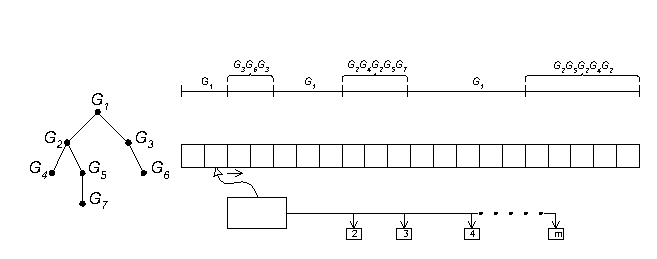
\includegraphics{img/pcgs/pocitad}
    \caption{Viacpočítadlový automat a tvar slova generovaného $treePCGS$}\label{pcgs_obr_pocitad}
  \end{figure}

  Vieme, že každá regulárna gramatika sa dá simulovať pomocou
  nedeterministického konečného automatu\footnote{pozri
  \cite{Hopc}}. Podobne budú v pravidlách nášho automatu $M$
  simulované pravidlá regulárnych komponentov $G_1,\dots ,G_m$. $M$
  bude používať svoje počítadlá $C_2,\dots ,C_m$ na zabepečenie
  toho, aby jednotlivé gramatiky $G_1,\dots ,G_m$ neboli simulované
  dlhšie ako to vyžaduje daná situácia (konfigurácia). V každej
  konfigurácii $M$ bude číslo $c(C_i)\; \forall i\in\{2,\dots ,m\}$
  uložené v $C_i$ uchovávať rozdiel medzi počtom prepisovacích
  krokov $G_i$ simulovaných $M$ a počtom prepisovacích krokov otca
  $G_i$ v stromovej komunikačnej štruktúre (to znamená, že ak $G_i$
  je požiadaná svojim otcom o vyprodukovanú vetnú formu, tak túto
  vetnú formu môže $G_i$ generovať najviac $c(C_i)$ krokov).
  \\ $M$ nedeterministicky striedavo simuluje gramatiky $G_1,\dots ,G_m$ a
  zároveň overuje, či slovo ge\-ne\-ro\-va\-né gramatikami je zhodné
  so slovom na vstupnej páske. Na začiatku $M$ simuluje $G_1$ a
  priebežne overuje vstupnú pásku. Zároveň po každom odsimulovanom
  prepisovacom kroku $G_1$ inkrementuje počítadlá všetkým synom
  $G_1$ a ostatné počítadlá zostanú nezmenené. Simulácia $G_1$
  skončí, keď $G_1$ vygeneruje komunikačný symbol $Q_i$ pre nejaké
  $i$. $M$ začne simulovať gramatiku $G_i$ z počiatočného
  neterminálu $S_i$. Počas tejto simulácie po každom prepisovacom
  kroku $G_i$ sa dekrementuje počítadlo $C_i$ a inkrementujú sa
  počítadlá všetkých sy\-nov $G_i$. Ak $G_i$ vyprodukuje terminálnu
  vetnú formu, tak $M$ zastaví a akceptuje vstupné slovo práve
  vtedy, keď bol vstup prečítaný až do konca. Ak $C_i$ je prázdne
  ($c(C_i)=0$) a $G_i$ v poslednom kroku vygeneroval na konci
  neterminál $A$, tak $M$ začne simulovať otca $G_i$ (v tomto
  prípade $G_1$) pričom pokračuje v prepisovaní z neterminálu $A$.
  Ak $G_1$ nemôže prepísať $A$ (t.j. nemá pravidlá na $A$), tak $M$
  neakceptuje vstupné slovo. Ak $G_i$ vegeneruje komunikačný symbol
  $Q_j$ pre nejaké $j$, tak $M$ začne simulovať $G_j$ (kde $G_j$ je
  synom $G_i$) z počiatočného neterminálu $S_j$. $M$ od tohto
  momentu po každom prepisovacom kroku $G_j$ dekrementuje $C_j$ a
  inkrementuje počítadlá všetkých svojich synov. $M$ takto
  rekurzívne simuluje gramatiky až kým poslená gramatika
  nevygeneruje terminálnu vetnú formu. \\ Z popisu práce $M$ by malo
  by zrejmé, že počet obratov je $2f(n)$ a počet testov na nulu je
  $f(n)$, lebo počítadlo $C_i$ začne klesať práve vtedy, keď je
  vygenerovaný komunikačný symbol $Q_i$. \\ Ak sa v pravidlách
  gramatík nenachádzajú žiadne $chain rules$\footnote{pravidlá typu
  $A\ra B$ kde $A,B$ sú neterminály}, tak $M$ pracuje v čase $n$. Ak
  sú v gramatikách takéto pravidlá, tak $M$ pracuje v čase $O(n)$,
  pretože existuje konštanta $d$ taká, že pre každé $w\in L(\Gamma)$
  existuje odvodenie, ktoré v každých $d$ krokoch vygeneruje aspoň
  jeden terminál.
\end{dokaz}

\medskip

Uvedomme si, že $m-1$ počítadlový automat vieme simulovať
viacpáskovým TS pracujúcim v rovnakom čase, a že počítadlá
uchovávajú čísla veľkosti najviac $n$,takže v binárnom kódovaní sa
zmestia do priestoru $O(\log n)$ Z týchto dvoch poznatkov plynie
nasledujúce tvrdenie.

\begin{veta}
  $\Langclass{treePCGS_m REG(f(n))}\subseteq NTIME(n)\cap NSPACE(\log
  n)$
\end{veta}

\begin{poznamka}
  Predchádzajúca veta nehovorí, že vieme zostrojiť ekvivalentný TS
  pracujúci v lineárnom čase a logaritmickom priestore. Hovorí len,
  že vieme zostrojiť ekvivalentný TS pracujúci v lineárnom čase a
  (iný) ekvivalentný TS pracujúci v logaritmickom priestore.
\end{poznamka}

Skúsme sa zamyslieť nad simuláciou $PCGS_mREG(f(n))$ priamočiaro
pomocou $m$-páskového TS. Ten by na každej páske simuloval
prepisovanie vetnej formy jednej gramatiky. Komunikácia medzi
gramatikami v tomto prípade znamená presunutie obsahu jednej pásky
na druhú. Keďže veľkosť pásky je $O(n)$ a komunikácií je $f(n)\in
O(n)$, tak časová zložitosť je $O(n^2)$. Pri takejto simulácii sa
nám ľahko môže stať, že nejaký kúsok vetnej formy bol presúvaný
medzi páskami $O(n)$ krát a nakoniec sa aj tak nedostal do
výsledného terminálneho slova. V nasledujúcej vete budeme toto
``zbytočné'' presúvanie eliminovať a dostaneme dobrý výsledok pre
$dagPCGS$.

\begin{veta}
  $\Langclass{dagPCGS_* REG} \subseteq NTIME(n)$
\end{veta}

\begin{dokaz}
  Nech $\Gamma=(N,K,T,G_1,\dots ,G_m)\in dagPCGS_mREG$. Chceme
  zostrojiť $m$-páskový\footnote{to znamená, že TS $A$ má $m$ hláv}
  nedeterministický TS $A$ pracujúci v lineárnom čase a akceptujúci
  jazyk $L(\Gamma)$.
  \\ V $\delta$-funkcii si $A$ uchováva pravidlá všetkých m gramatík
  a v stavoch si drží aktuálne neterminály\footnote{keďže gramatiky
  sú regulárne, vo vetnej forme danej gramatiky sa vyskytuje najviac
  jeden neterminál} všetkých gramatík. Na páskach $T_1,\dots ,T_m$
  sú vetné formy generované gramatikami $G_1,\dots ,G_m$ alebo $T_i$
  obsahuje blank symbol $B$, ak sa $A$ nedeterministicky rozhodne,
  že vetnú formu, ktorú generuje $G_i$ sa neobjaví vo výslednom
  terminálnom slove generovanom $\Gamma$ t.j eliminovanie
  \mbox{``zbytočných''} presúvaní z jednej pásky na druhú.
  \\ Na začiatku bude $A$ v stave so začiatočným neterminálom pre
  každú gramatiku. Pre každé $i=1..m$ $A$ uhádne, či sa vetná forma
  generovaná gramatikou $G_i$ bude nachádzať vo výslednom
  terminálnom slove. Ak $A$ rozhodne, že vetná forma generovaná
  $G_i$ bude vo výslednom slove, tak $A$ bude simulovať odvodenie
  gramatiky $G_i$ na páske $T_i$. Ak $A$ rozhodne, že nebude, tak
  $A$ zapíše na pásku $T_i$ symbol $B$ a ďalej nesimuluje odvodenie
  $G_i$ na páske $T_i$. Takto $A$ simuluje iba to, čo sa vo
  výslednom slove naozaj objaví.
  \\ Jeden krok simulácie $A$ pozostáva z jedného prepisovacieho kroku
  každej z gramatík, pre ktoré sa $A$ rozhodol, že ich bude
  simulovať. To môžeme, lebo ako sme si povedali $A$ si v stave
  uchováva aktuálne neterminály každej z gramatík. Takto $A$
  pokračuje, až kým sa na páske $T_1$ neobjaví terminálne slovo,
  alebo až kým sa aspoň na jednej páske neobjaví $query$ symbol. \\
  Ak sa na $T_1$ objaví terminálne slovo, tak $A$ porovná obsah
  pásky $T_1$ so vstupom a ak sa rovnajú, tak $A$ akceptuje vstupné
  slovo.

  Ak aktuálny neterminál $G_i$ je $Q_j$ a
  \begin{itemize}
    \item ani $T_i$ ani $T_j$ neobsahuje $B$, tak $A$ prekopíruje obsah
    $T_j$ na miesto $Q_j$ na páske $T_i$ a celý obsah pásky $T_j$
    prepíše na $S_j$ (počiatočný neterminál gramatiky $G_j$). Po tomto
    pokračuje $A$ v simulácii $G_i$ z neterminálu, ktorý bol posledným
    symbolom pri kopírovaní. $A$ uhádne, či ďalšia vetná forma
    generovaná $G_j$ bude časťou výsledného slova alebo nie. Podľa
    toho začne simulovať $G_j$ z počiatočného neterminálu $S_j$ alebo
    na $T_j$ zapíše $B$.
    \item buď $T_i$ alebo $T_j$
    obsahuje $B$, tak to znamená, že $A$ uhádol nesprávne\footnote{Ak
    $T_j$ obsahuje $B$, tak $T_i$ sa objaví vo výsledku, a teda aj
    $T_j$ bude vo výsledku, keďže si ju $G_i$ vyžiadala, teda $A$ zle
    uhádol. Ak $T_i$ obsahuje $B$, tak $T_j$ sa má objaviť vo
    výsledku, ale nemá sa ako dostať cez $T_i$, takže $A$ zle uhádol.} a
    výpočet sa zasekne.
    \item $T_i$ aj $T_j$ obsahuje $B$, tak $A$ nezmení obsah $T_i$ a
    nedeterministicky uhádne, či sa ďalšia vetná forma generovaná
    $G_j$ objaví vo výslednom terminálnom slove. Podľa toho $A$ začne na
    $T_j$ simulovať $G_j$ od počiatočného neterminálu $S_j$ alebo na
    $T_j$ nechá $B$.
  \end{itemize}
  Ak sa naraz na viacerých páskach objavia komunikačné symboly, tak
  $A$ kopíruje vetné formy v určitom poradí tak, aby nekopíroval
  nejaký komunikačný symbol. To sa určite dá, pretože uvažujeme
  komunikačnú štruktúru $dag$, ktorá nepripúšťa cykly. \\ Pre každé
  slovo $w\in L(\Gamma)$ existuje postupnosť správnych
  nedeterministických rozhodnutí TS $A$, ktorá vedie k odvodeniu
  tohto slova na páske $T_1$. Keďže komunikačná štruktúra nepripúšťa
  cykly, tak každý symbol akceptovaného slova $w$ bol kopírovaný z
  jednej pásky na druhú najviac $m-1$ krát, čo je konštantne veľa.
  Teda na prekopírovanie všetkých symbolov slova $w$ potrebujeme čas
  $O(n)$. Na páskach generujeme iba symboly, ktoré sa objavia vo
  výslednom slove $w$, teda na vygenerovanie všetkých symbolov slova
  $w$ potrebujeme čas $O(n)$. Konečne na porovnanie terminálneho
  slova na páske $T_1$ so vstupom potrebujeme čas $O(n)$. Teda
  celkovo pracuje $A$ v čase $O(n)$.
\end{dokaz}

\medskip

Uvedieme ešte niekoľko tvrdení, ktoré hovoria o tom, že ani
zvýšenie počtu gramatík, ani zvýšenie počtu komunikačných liniek v
stromovej štruktúre nedokáže vykompenzovať obmedzenie počtu
komunikačných krokov.

\begin{veta}
  $\Langclass{centrPCGS_2 REG(n)} - 
    \Langclass{treePCGS_* REG(f(n))} \neq\emptyset$
  pre $f(n)\not\in\Omega (n)$
\end{veta}

\begin{dokaz}
  Uvedieme\footnote{podrobnosti možno nájsť v \cite{some}} len, že
  dôkaz uvažuje jazyk \newline \centerline{$L=\{
  a^{i_1}b^{i_1}a^{i_2}b^{i_2}\dots a^{i_k}b^{i_k}c\mm k\geq 1,
  i_j\geq 1\; pre\; j\in\{ 1,\dots ,n\}\}$} o ktorom sa ukáže, že
  $L \in \Langclass{centrPCGS_2 REG(n)}$ a
  $L \not\in \Langclass{treePCGS_* REG(f(n))}$. Využíva sa pri tom
  simulácia $treePCGS_mREG(f(n))$ pomocou $m-1$ počítadlového
  automatu ako to bolo uvedené vo vete \ref{pcgs_veta_multicounter}.
\end{dokaz}

\begin{veta}
  Pre $f(n)\not\in\Omega (n)$ platí:
  \begin{itemize}
    \item $\Langclass{one-way-array PCGS_m(f(n))} \subsetneq
          \Langclass{one-way-array PCGS_m(n)}$
    pre $m\geq 2$
    \item $\Langclass{centrPCGS_m(f(n))} \subsetneq
      \Langclass{centrPCGS_m(n)}$
    pre $m\geq 2$
    \item $\Langclass{treePCGS_m(f(n))} \subsetneq
      \Langclass{treePCGS_m(n)}$
    pre $m\geq 2$
  \end{itemize}
\end{veta}

\begin{veta}
  $\Langclass{centrPCGS_{k+1}(k)}-\Langclass{treePCGS_*(k-1)}\neq\emptyset$
  pre ľubovoľnú konštantu $k$.
\end{veta}

\begin{veta}
  Pre ľubovoľné $k\geq 1$ a ľubovoľné
  $x\in\{centr,tree,one-way-array\}$ platí:
  \begin{itemize}
    \item
    $\Langclass{xPCGS_{k+1}(k-1)}\subsetneq\Langclass{xPCGS_{k+1}(k)}$
    \item $\Langclass{xPCGS_*(k-1)}\subsetneq\Langclass{xPCGS_*(k)}$
  \end{itemize}
\end{veta}

\section{Niektoré ďalšie vlastnosti $PCGS$}

\begin{veta}
  $\Langclass{PCGS_* CF}$ je úplná $AFL$.
\end{veta}

\begin{veta}
  $centrPCGS_*CF {<_4}^{Var} CF$
\end{veta}

\begin{veta}
  $centrPCGS_*CF {<_4}^{Prod} CF$
\end{veta}
